
\section{Layout of the Endcap Petal}

Figure~\ref{endcap_model} depicts the endcap petal model used for calculating thermal impedances.

\begin{figure}[ht!]
\begin{center}
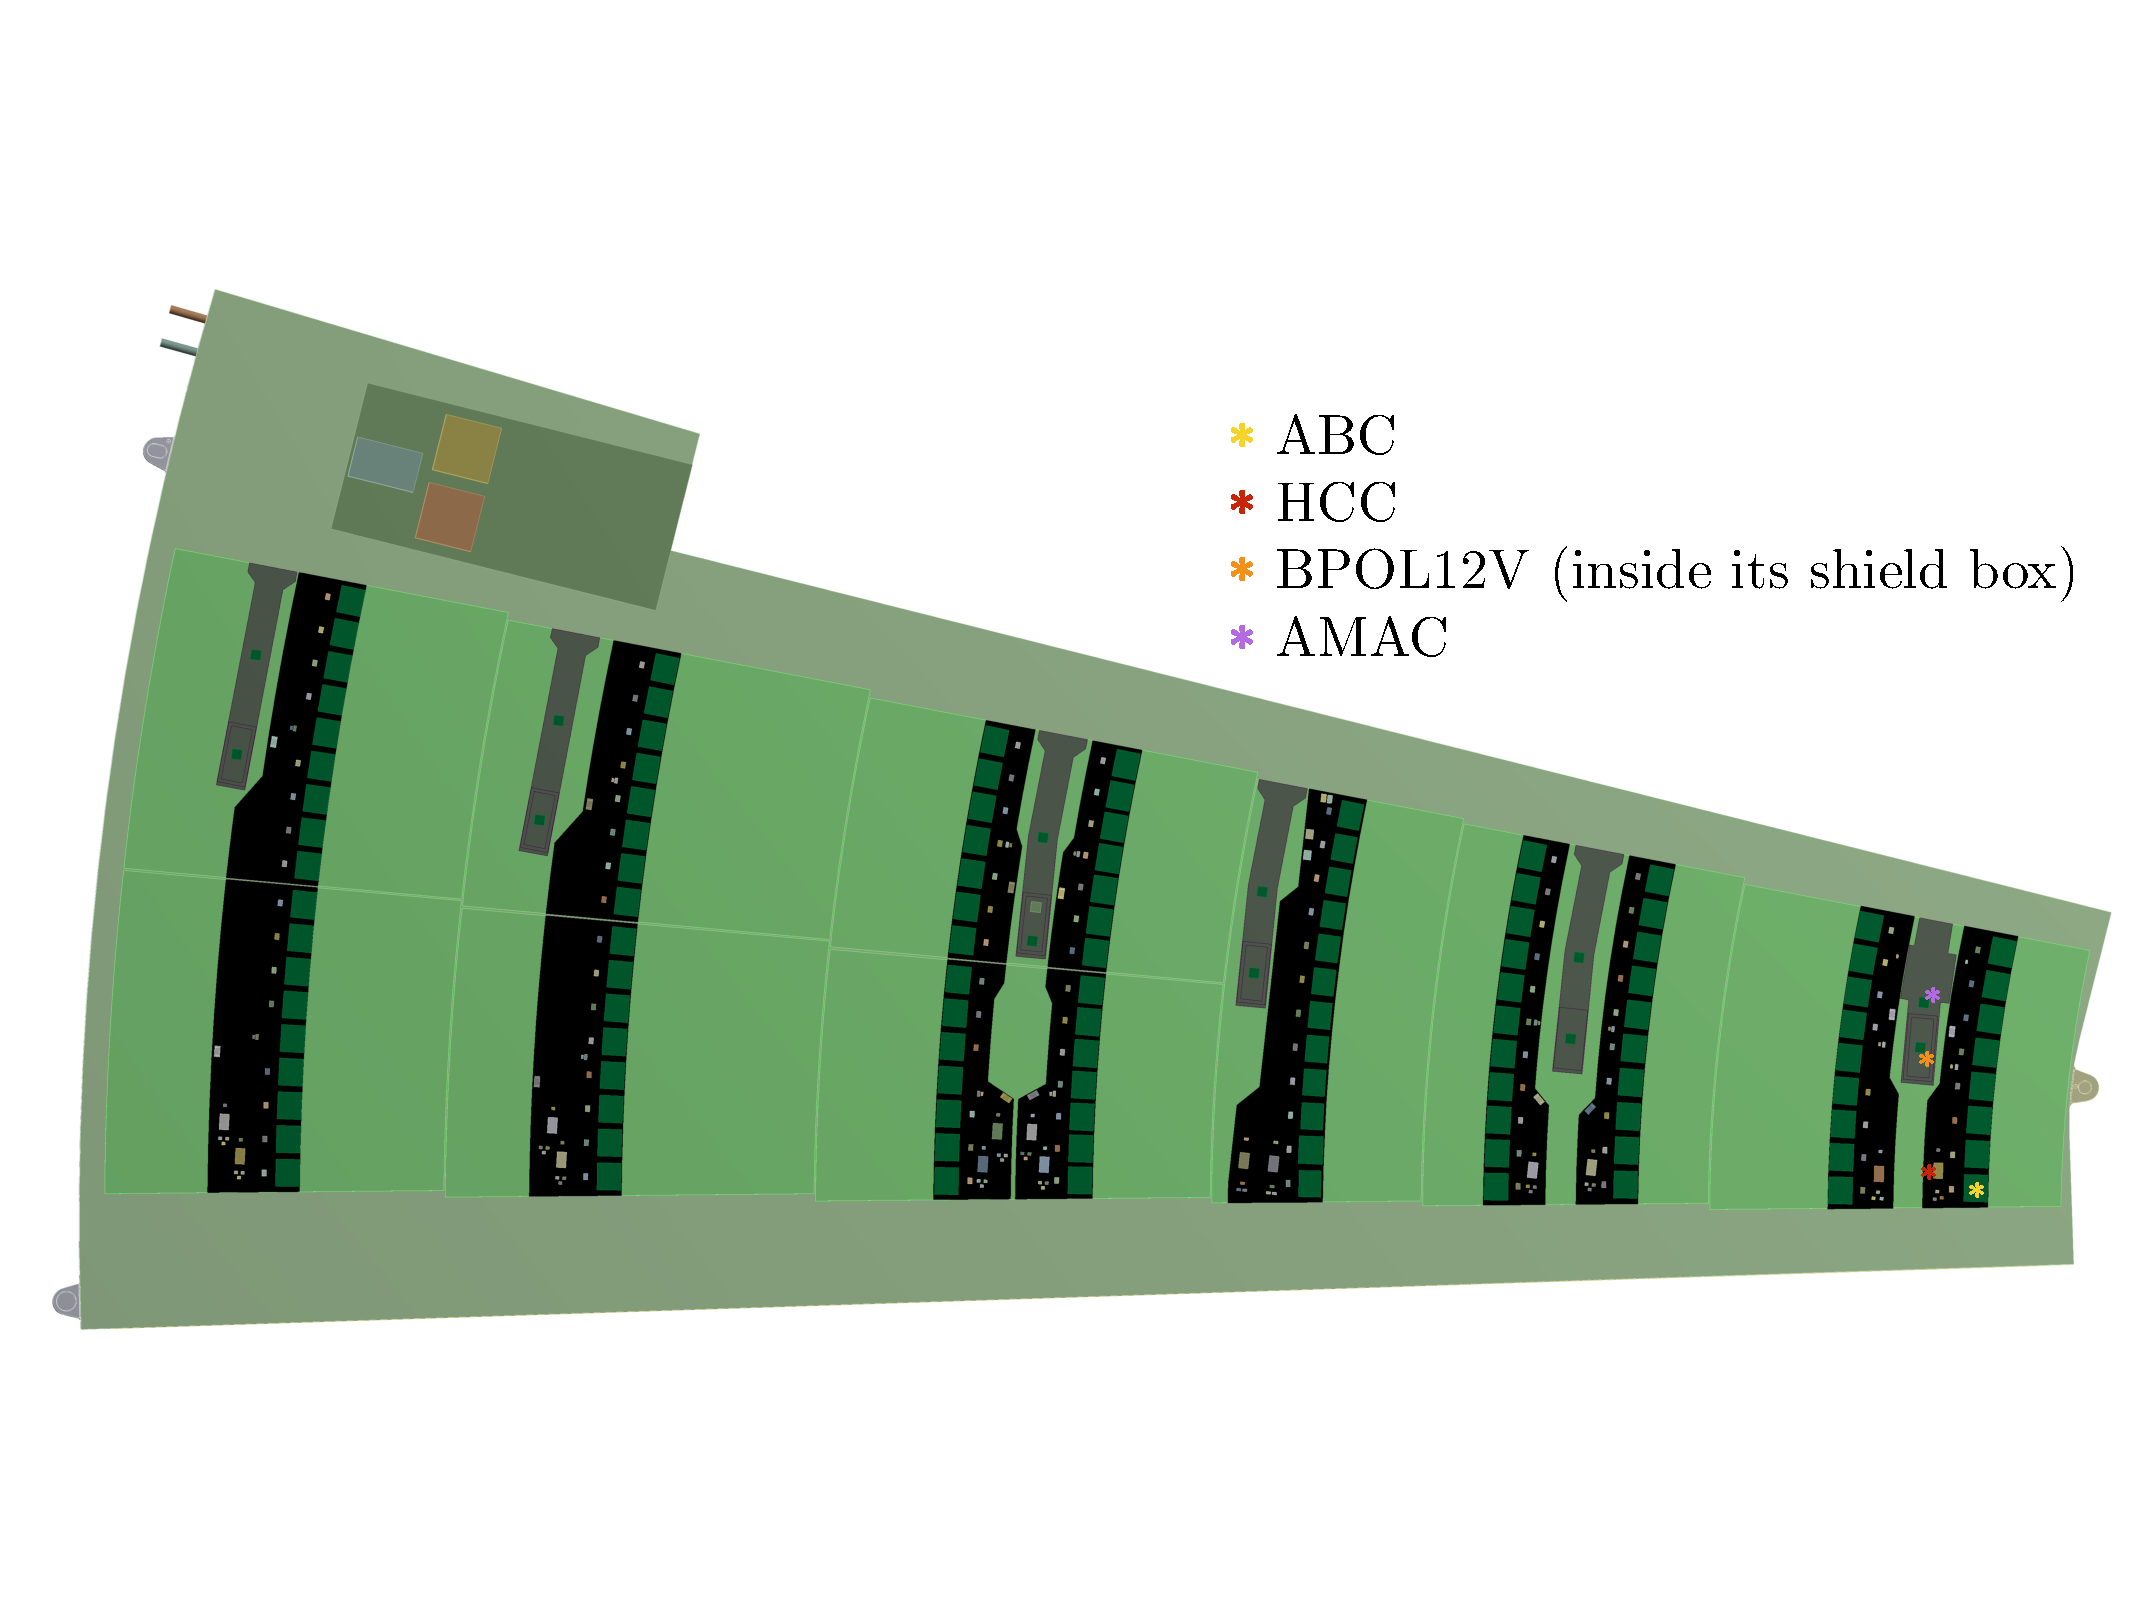
\includegraphics[width=0.99\linewidth]{figures/m30C_0Wm2C_Setup_BPOL12V.pdf}
\end{center}
\caption{The endcap petal model used for extracting thermal impedances. The front-end components are
labeled in R0 (the rightmost module).}
\label{endcap_model}
\end{figure}

The number of BPOL12Vs, AMACs, ABCs, HCC, and the sensor area of each module are listed in
Table~\ref{tab:layout_parameters}.
%
\let\arraystretcha\arraystretch
\renewcommand\arraystretch{1.1} % 1.6
\begin{table}[h]
\begin{center}
\adjustbox{max width=\textwidth}{ %% just before tabular
\begin{tabular}{|l|r|r|r|r|r|r|} \hline
Module & nBPOL12V & nAMAC & nABC & nHCC & Sensor area (cm$^2$) \\ \hline
R0     &      1 &     1 &   17 &    2 &                 92.0 \\
R1     &      1 &     1 &   21 &    2 &                 91.0 \\
R2     &      1 &     1 &   12 &    2 &                 76.0 \\
R3     &      2 &     2 &   28 &    4 &                164.0 \\
R4     &      1 &     1 &   16 &    2 &                178.0 \\
R5     &      1 &     1 &   18 &    2 &                186.0 \\
\hline \end{tabular}
} %% resizebox after tabular
\end{center}
\caption{Number of components on each module.}
\label{tab:layout_parameters}
\end{table}
\let\arraystretch\arraystretcha

